\subsubsection{Fluid Flow on Continental Margins, GIS \& visualisation}
\index{Unnithan, Vikram}

\paragraph{Research Team}
Vikram Unnithan (Professor), Angela Sch\"{a}fer (Research Associate)\\
Yangze Fu (PhD Student),
Jakob Hauschildt (PhD student\footnote{Joachim Vogt \& Vikram Unnithan - joint
PhD supervisors}), Hannes Wagner (PhD student\footnote{Vikram Unnithan - second
PhD supervisor}), Birte-Marie Ehlers (PhD student\footnote{Vikram Unnithan - joint PhD
supervisor}), Angelica Garcia (Phd student\footnote{Angela Sch\"{a}fer \&
Vikram Unnithan - joint supervision}),  Anke Lederer (Diploma student\footnote{Angela Sch\"{a}fer \&
Vikram Unnithan - joint supervision}), Florian Neu (IT technician) \\

The research group fits into three broad categories of marine geophysics and Geographic Information Science (GIS):
(a) Understanding and modelling fluid flow processes on continental margins. The aim is to provide a better
quantification of fluid (hydrocarbon) transport processes from the deeper geosphere to the shallower biosphere.
Current research topics include quantification of the role and influence of heat budgets on fluid transport,
gas hydrate modelling and numerical hydrate simulations.(b)The second area of research is seismic interpretation
and petroleum system's modelling of continental margins offshore Norway and Ireland. This research forms part
of the ongoing work within the framework of the International Research Consortium on Continental Margin (IRCCM). (c)The
third focal area is geoinformatics, GIS and scientific visualisation. Of particular interest is the  development
 of GIS methodologies, conceptual frameworks and techniques (MarineXML, SensorML) to capture, manage and analyse large volumes of real-time geodata.

% 150 words about research in general

\paragraph{Highlights}


% 500 words about highlights in 2006 % gravity modelling from the ionian and magnetics -start ..
%Research and assessment of potential gas hydrate and associated features and theoretical


%During the past year, my modelling research has concentrated on three aspects of fluid flow on continental margins: 1.) mathematical or theoretical modelling, 2.) petroleum system's modelling and 3.) seismic modelling

In terms of collaborations and new projects, 2006 has been an extremely successful year.
 The research group has also grown with the addition of PhD students and support staff.

Yanzhe Fu has started his PhD thesis using conventional 2D and 3D seismic data as a basis for seismic interpretation, attribute modelling and petroleum system's modelling of the Norwegian and Irish margins. Seismic interpretation software Charisma (donated by Schlumberger) and SMT provide the necessary tools for this type of modelling and interpretation. Petroleum system's modelling includes and involves the generation, migration and accumulation of hydrocarbons. Both study sites are not only active hydrocarbon producing regions, they also contain numerous shallow fluid-flow related features.

An assessment of potential occurrence of gas hydrates and associated features and a theoretical understanding of hydrate formation and dissociation is particularly important with regard to geo-hazard analysis, climate modelling and fluid flow processes on continental margins. The 1D and 2D dynamic modelling of the hydrate system and associated fluid flow is the subject of Jakob Hauschildt's PhD work.  This thesis is jointly supervised by Joachim Vogt and myself. Research on the gas hydrates also deals with the production of excess (over)pressure beneath impermeable hydrate layers. The formation of fractures by overpressures is the subject of a modelling exercise. The ability to simulate hydrofracturing is new in this type of petroleum basin modelling. This work is in collaboration with Prof. V. Spiess, University Bremen and aims to model hydrate formation and fracturing of subsurface layers, and compare the results with seismic data.

Static hydrate modelling of the Irish Atlantic margin, Mediterranean and in particular the Ionian Sea have been carried out in joint collaboration with Dr. Praeg. The results have provided interesting insights into the total volume and thickness of hydrates in these regions. The impact of differing glacial-interglacial scenario's on the local geomorphology and the potential geo-hazard risk were presented at the Applied Geophysics Union meeting this fall in San Francisco.

The modelling efforts are complemented by the observational side by providing the framework for understanding processes, postulating and testing hypothesis. During 2006, the group has been involved in various ongoing projects such as HERMES, NEPTUNE and planning future projects such as ESONET. One of the key sites for the establishment of such a long-term, internet-connected observatory is Tjarno, Sweden. This site is also of interest for Statoil, since it provides easy access to study the environmental impact of hydrocarbon activities and monitor changes in the biological community. Within these projects, the group is involved in cold water coral research, benthic habitat mapping, video photomosaicing and GIS. Data management applications in terms of geodatabase servers and Web Map Services are permanently extended, improved and maintained to develop a coherent concept for 'Integrated web-based mapping and data management for large-scale international projects'.

\begin{figure}[ht]
  \begin{center}
    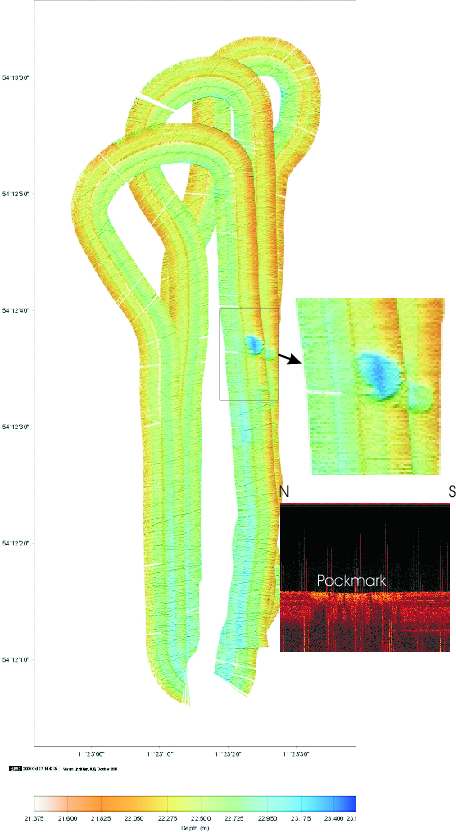
\includegraphics[width=6cm]{Unnithan/prof-unnithan-fig1}
    \caption{Preliminary multibeam results from the Alkor Cruise showing the location of the large pockmark and highlighting the intense trawling activity in the region. The two enlarged sections are a.) detail of the pockmark, and b.) N-S parametric echosounder profile. {\em Data courtesy of Prof. Spiess, processing and interpretation was performed at IUB by Vikram Unnithan.}}
    \label{fig:prof-unnithan}
   \end{center}
\end{figure}

In September 2006, I participated in a short geophysical research
cruise to the Baltic Sea.
 The general purpose of this excursion was to test equipment and investigate shallow fluid flow structures
 on the seabed. The discovery of a large pockmark was the highlight of this cruise (Fig~\ref{fig:prof-unnithan}). Preliminary interpretation suggests that this structure is probably linked to shallow biogenic methane production and the underlying geological formations.

The storage and archiving of huge data volume needs a comprehensive and integrated data management strategy flexible enough to meet the changing demands of users, technology and digital standards. Current research, focuses on developing a system based on MarineXML (eXtended Markup Language), which provides direct analysis and long-term storage in relational databases. Since most large geoscience relational databases deal with
geo-coded vector data, a new concept is being developed for integrating image or raster data. The analysis of such geocoded data is facilitated by GIS. Strategies to deal with real-time data from the seabed observatories have been tested during the past year using WebGIS. Different implementations, especially open source were deployed for the HERMES project by Anke Lederer (Diploma student).

%This is of particular interest Web GIS Anke Lederer .. The spatial and temporal analysis of geo-data is critical for understanding continental margin processes. Geographic Information System (GIS) is a broad field that deals with the analysis, processing and visualisation of geoscience related data.
%Conferences - Multibeam,
%WebGIS
%- start PhD students, plus other ..
%- presentation to the IES group ..



\paragraph{Organization}
% list the (research) events you have organized, if any,

\begin{enumerate}
\item GIS workshop (January 2006) for IUB undergraduates and HERMES postgraduates (external PhD students).
\item Angela Sch\"{a}fer teaches and organises the GIS module (September 2006) at the annual summer university "Informatica Feminale" in Bremen.
%And that we counsel other intituts and projekt in terms of GIS settings and Geodatabase building
\end{enumerate}

\paragraph{Collaborations}
\noindent

Regional:
\begin{enumerate}
\item {\sl Wasser- und Schifffahrtsamt Bremen}
\item {\sl University Bremen} \\ Prof. V. Spiess
\item {\sl Alfred Wegener Institute} \\ Dr. W. Jokat
\item {\sl IUB} \\ Prof. P. Baumann and GeoAstro faculty
\item {\sl ATLAS Elektronik GmbH } \\ Prof. M. Siegel
\item {\sl World Data Center MARE maintained by the Alfred Wegener
Institute for Polar and Marine Research (AWI) and the Center for
Marine Environmental Sciences MARUM at University Bremen} \\
Dr. M. Diepenbroek and Dr. H. Grobe
\end{enumerate}

National:
\begin{enumerate}
\item {\sl DFG Priority-Program 1144 \& World Data Center
MARE/PANGAEA}
\item {\sl Schlumberger GmbH} \\ A. Glocke
\item {\sl Integrated Exploration Services Gmbh} \\ Prof. D. Welte
\end{enumerate}

International:
\begin{enumerate}
\item {\sl EU-project HERMES}
\item {\sl Istituto Nazionale di Oceanografia e di Geofisica Sperimentale (OGS), Trieste, Italy} \\ Daniel Praeg and Silvia Ceramicola
\item {\sl Indian Institute of Technology, Madras, India} \\ Prof. A. Subramaniam
%\item Indian Ambassador
%\item JNU subramaniam
\end{enumerate}

\paragraph{Grants }
% list the running grants in 2005, if none have been received, please delete this
% subsection.

\begin{enumerate}

\item
Funded by EU, \emph{HERMES}, WP leader, P.I. Prof. L. Thomsen, (April 2005 -  March 2009) 

\item
Funded by private industry, \emph{IRCCM observatory}, coordinator Prof. L. Thomsen, EU/US,
(January 2006 - December 2008) 

\item
Funded by Private Industry Statoil, \emph{CORAMM}, coordinator Prof. L. Thomsen, (October
2006 - May 2010) 
\end{enumerate}



\paragraph{Awards, Prizes}
% list the grants you have received in 2005, if none have been received, please delete this
% subsection.
\begin{enumerate}
\item {RCOM, University Bremen} ``Yangze Fu received the Best Geosciences Master's Thesis award, University Bremen''
\end{enumerate}

%Publications should be delivered as a separate file (naming convention profxxx.bib. See description by R. Helling. Please make sure that all your publications are referred to in the TeX file. This can either be in form of a \cite{profxxxkey} or as a \nocite{profxxxkey} in the end. A publication which is not reffered to on the LaTeX file doesn't produce any output in the report.
% Euronews .. documentary ..
% publications - AGU, EGU ..


\nocite{ceramicola2}
\nocite{praeg1}



% Daniel Praeg, Vu, \& Camerlenghi, A. 2006. Gas hydrate stabilty and prospectivity in the med sea, results from hydramed .. Fifth international workshop on methane hydrates reaserch, 9-12 Oct.
% Eurodom meeting in Trieste, networks, talks ..
